\subsection{Stopped Kaon}
In this section , we compare some quantities of data and MC simulation that K stop in the liquid argon detector and can detect stopped point.
Figure \ref{cHitq_hough}-\ref{cPrimaryCharge_hough} shows Data and MC comprison for signal hit charge , sigmal width , cluster charge and primary paricle charge distribution.
Data of signal charge and signal width are consistnt with MC one in error by less than two $\%$ and data of cluster charge and parimary charge are consistent with  MC one in error by less than five $\%$.
\begin{figure}[htbp]
  \begin{minipage}{0.5\hsize}
    \begin{center}
      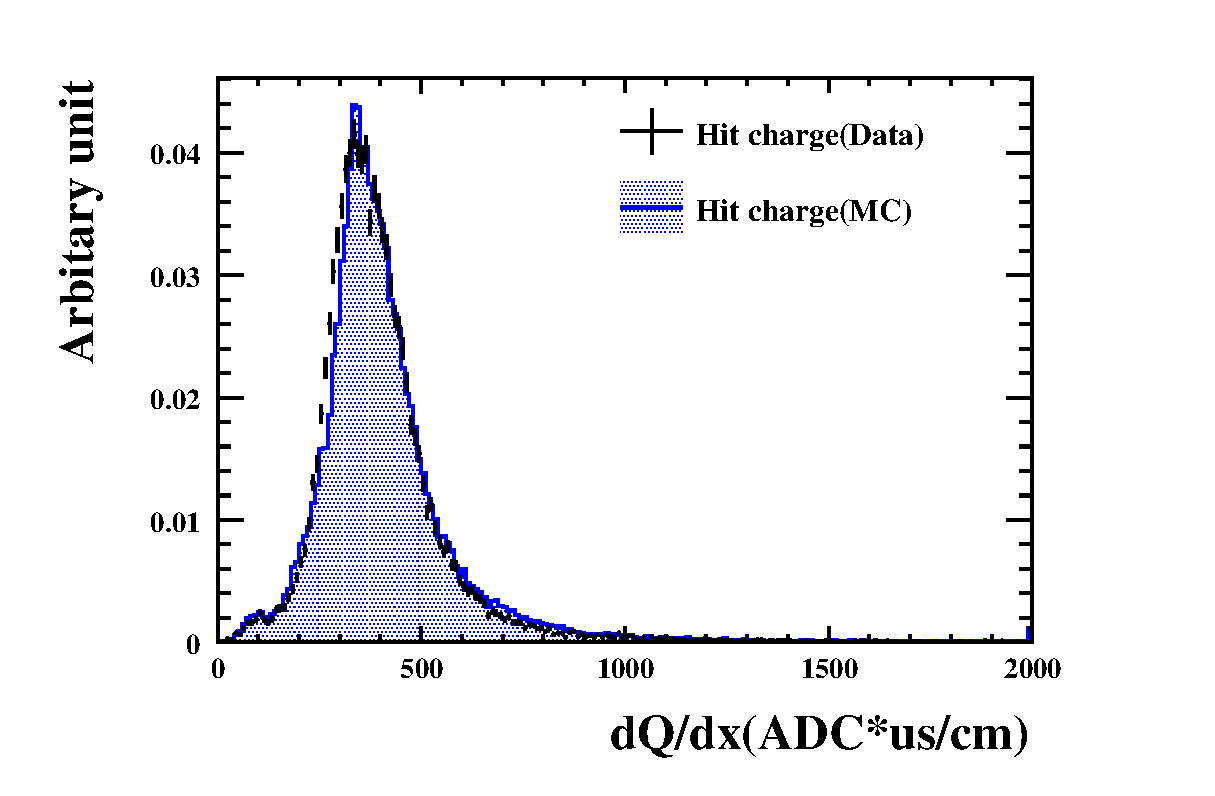
\includegraphics[width=50mm]{fig/cHitq_hough.eps}
    \end{center}
    \caption{Data-MC comparison for hit charge in all range}
    \label{cHitq_hough}
  \end{minipage}
  \begin{minipage}{0.5\hsize}
    \begin{center}
      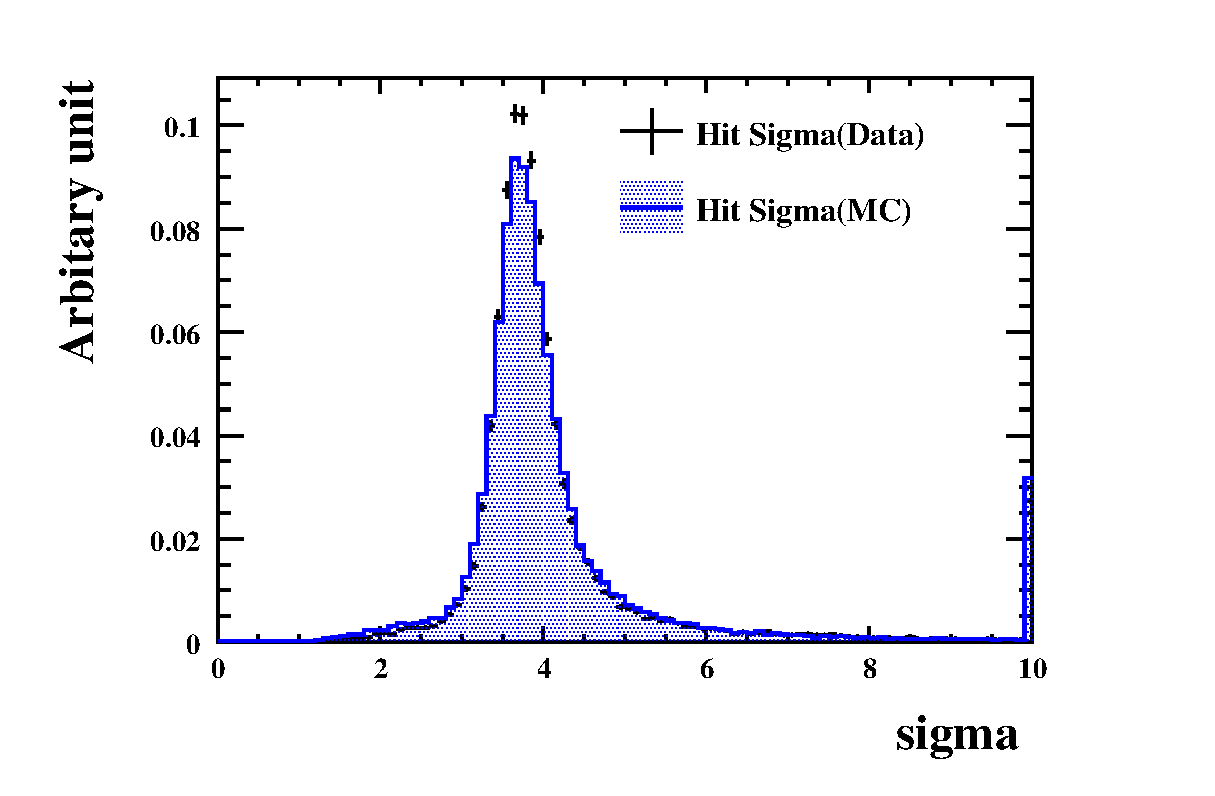
\includegraphics[width=50mm]{fig/cHitSigma_hough.eps}
    \end{center}
    \caption{Data-MC comparison for hit sigma in all range}
    \label{cHitSigma_hough}
  \end{minipage}
\\
  \begin{minipage}{0.5\hsize}
    \begin{center}
      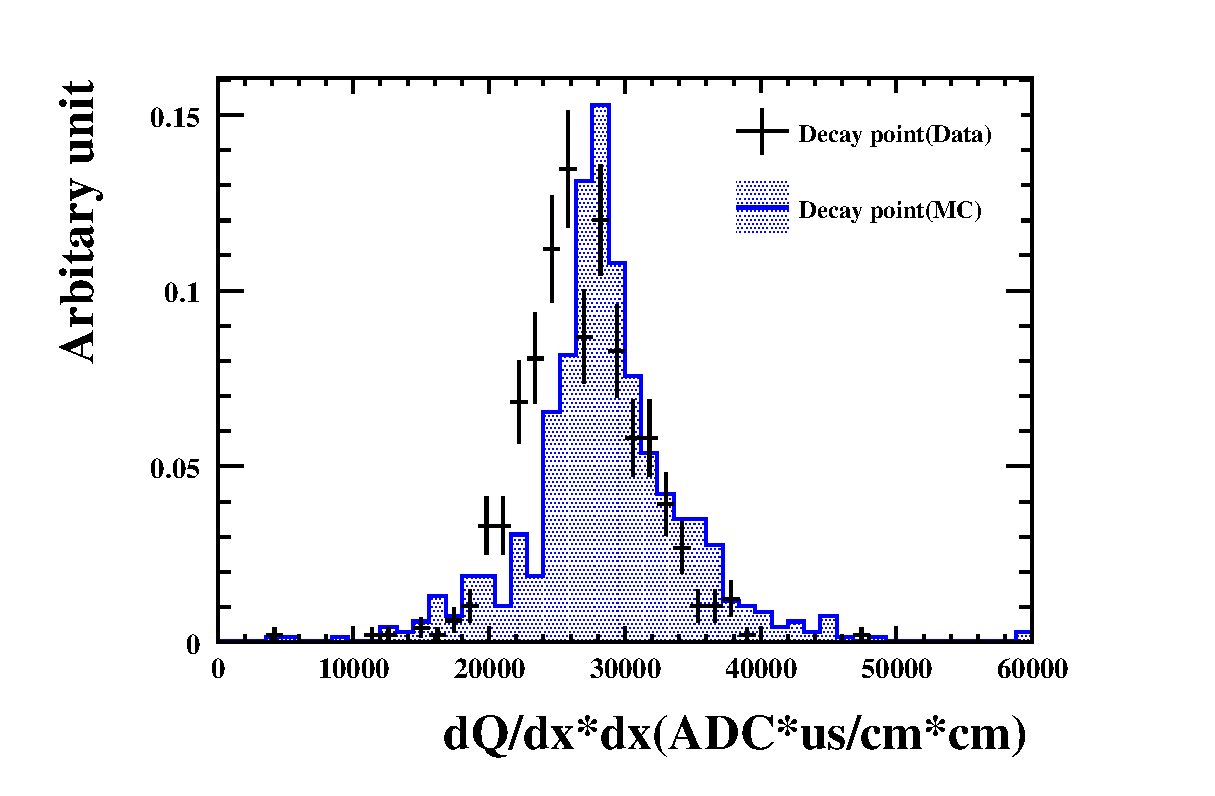
\includegraphics[width=50mm]{fig/cClusterCharge_hough.eps}
    \end{center}
    \caption{Data-MC comparison for Cluster Charge}
    \label{cClusterCharge_hough}
  \end{minipage}
  \begin{minipage}{0.5\hsize}
    \begin{center}
      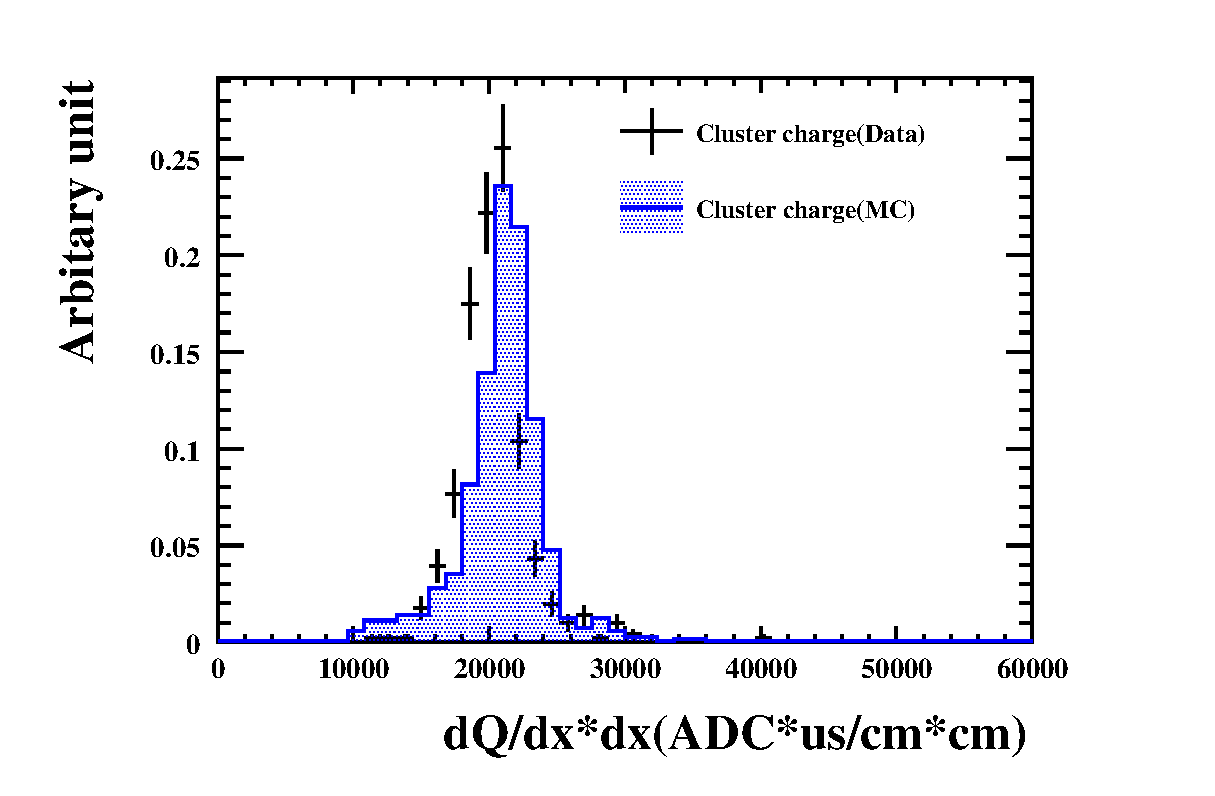
\includegraphics[width=50mm]{fig/cCSTSP_hough.eps}
    \end{center}
    \caption{Data-MC comparison for Primary particle charge}
    \label{cPrimaryCharge_hough}
  \end{minipage}
\end{figure}
 \\

Figure \ref{cq27_hough} shows signal hit charge distribution of restricted channel 27. 
As it can be noiced for figure \ref{cq27_hough} , signal charge have two peaks at 300 and 500 dQ/dx.
Because two peaks has correlation of $\Delta$TOF , there is some possibility of not passig in the center of the detector.
So , we use only the event that signal charge of restricted channel 27 is less than 350.
Figure \ref{RangeVsHit_hough} shows signal hit charge distribution in different distance from the stopped point.

\begin{figure}[!htb]
  \begin{center}
    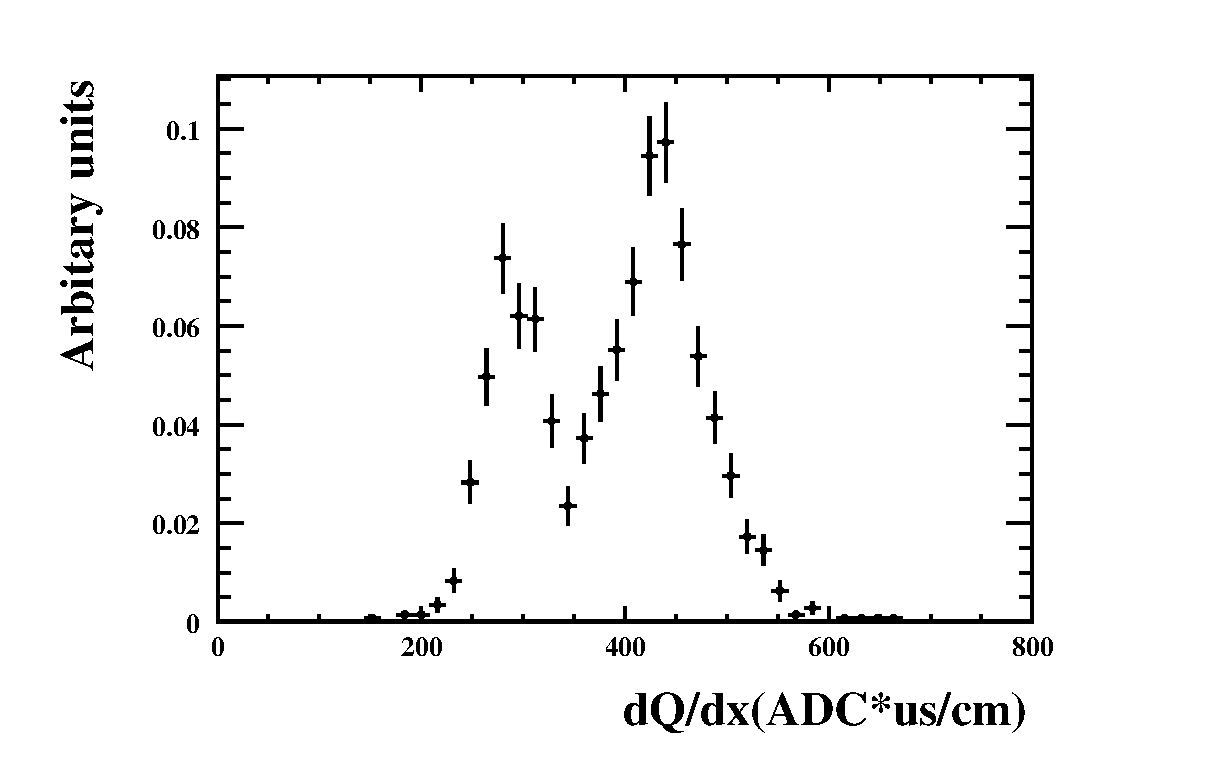
\includegraphics[width=70mm]{fig/cq27_hough.eps}
  \end{center}
  \label{cq27_hough}
  \caption{Hit charge in channel 27}
\end{figure}

\begin{figure}[!htb]
  \begin{center}
    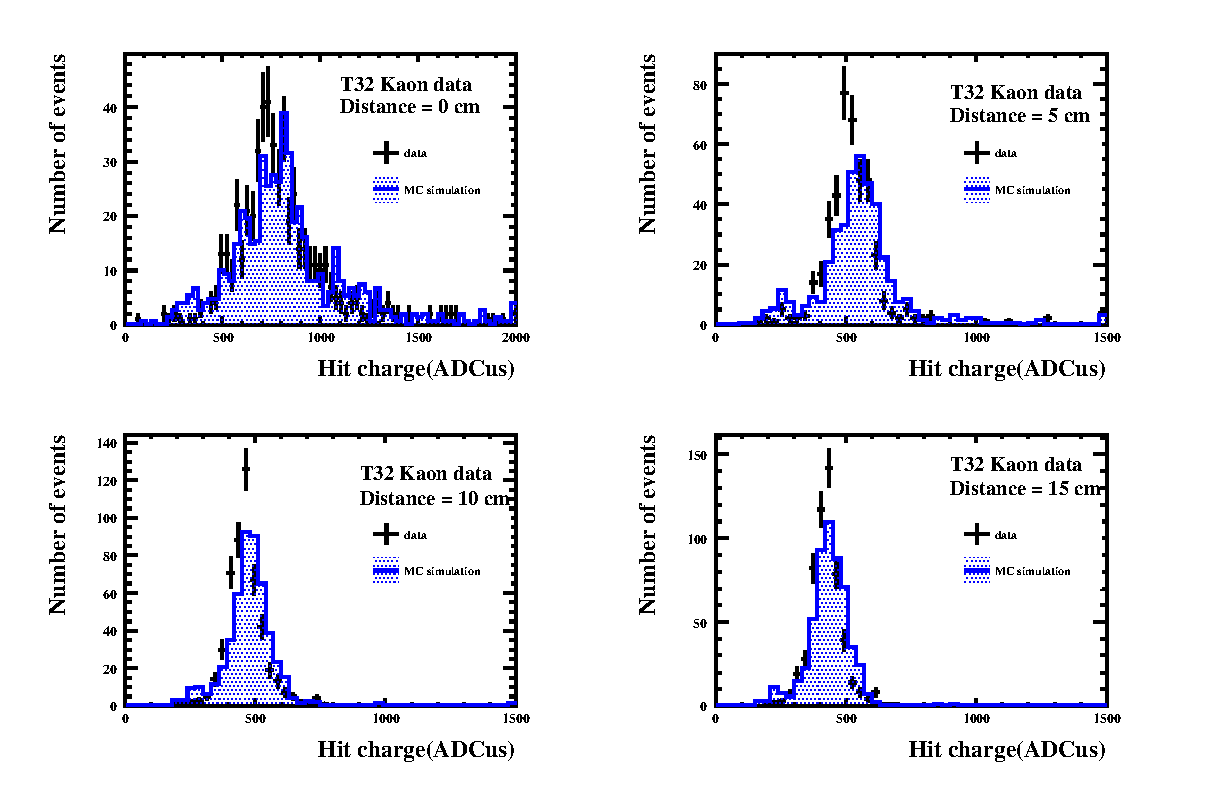
\includegraphics[width=100mm]{fig/RangeVsHit4_wcut_hough.eps}
  \end{center}
  \caption{Data-MC comparison for hit charge distribution in different distance from the stopped point(top left:decay point,top light:decay point-5cm,bottom left:decay point-10cm,decay point-15cm)}
  \label{RangeVsHit_hough}
\end{figure}

As it can be noticed for figure \ref{RangeVsHit_hough} , data plot is consistent with MC one.
Figure \ref{RangeVsHitRatio_hough} shows data/MC ratio of signal hit charge distribution in different distance from the stopped point.
Data of signal charge in dirfferent distance from stoppd point are consistnt with MC one in error by less than five $\%$ 

\begin{figure}[htb]
  \begin{center}
    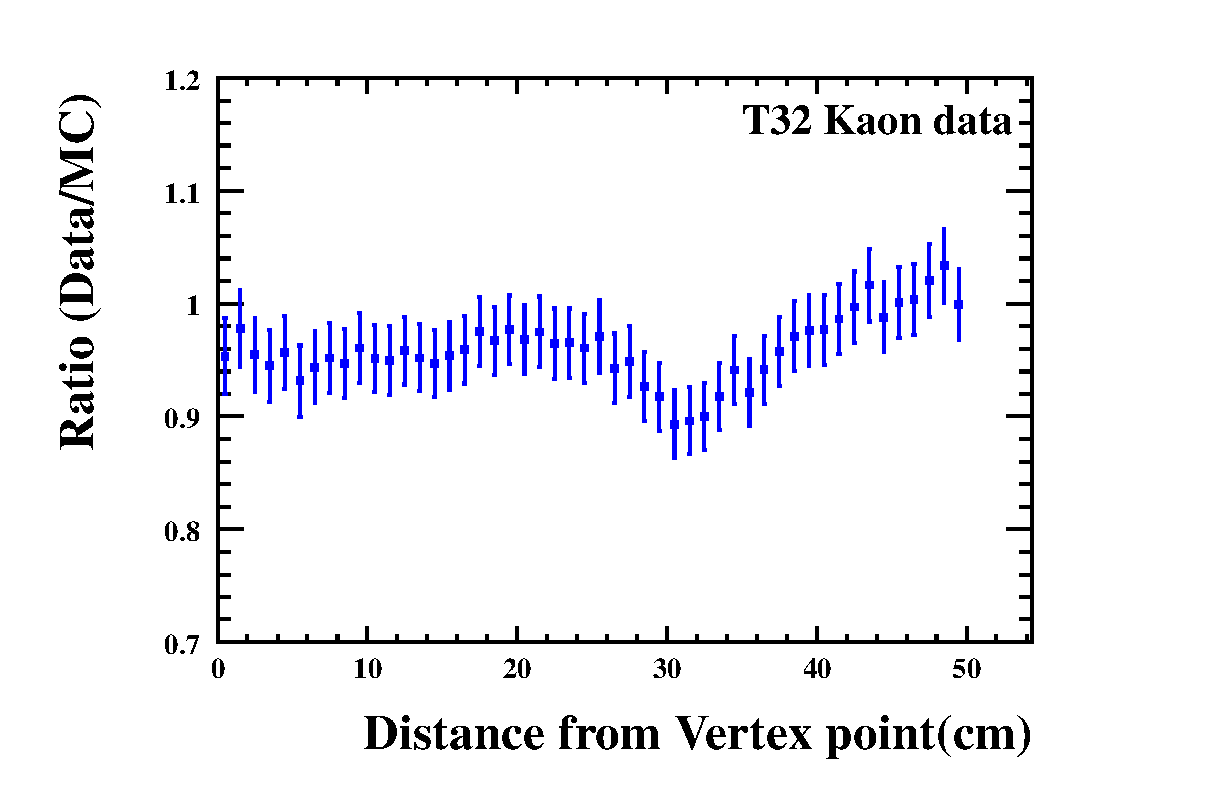
\includegraphics[width=70mm]{fig/RangeVsHitRatio_wcut_hough.eps}
  \end{center}
  \caption{Data/MC ratio for hit charge distribution in different distance from the stopped point}
  \label{RangeVsHitRatio_hough}
\end{figure}



